%%%%%%%%%%%%%%%%%%%%%%%%%%%%
% Este documento pertence à classe cls-PFC-COEEL.cls
% NÃO ALTERE NADA AQUI
%%%%%%%%%%%%%%%%%%%%%%%%%%%%
%
% Apenas para PFC
%
\ifpfc % se é PFC
   \include{./PFC_Especificos/j_Consideracoes_Finais}
   \include{./PFC_Especificos/k_Sugestoes_Trab_Futuros}
\fi 
%
%%%%%%%%%%%%%%%%%%%%%%%%%%%%%%
%%%%%%%%%%%%%%%%%%%%%%%%%%%%
%%%% CRONOGRAMA
%
% Apenas para Pré-Projeto
%
\ifpreprojeto % se é Pré-Projeto
   %%%%%%%%%%%%%%%%%%%%%%%%%%%%%%%%%%%%%%%%
%
% o CRONOGRAMA é obrigatório 
% APENAS PARA PRÉ-PROJETO de PFC
%
%%%%%%%%%%%%%%%%%%%%%%%%%%%%%%%%%%%%%%%%

\chapter{CRONOGRAMA}

O cronograma deste trabalho está organizado em fases que abrangem desde a pesquisa teórica até a implementação prática do projeto. A primeira etapa consiste no levantamento bibliográfico e estudo dos fundamentos teóricos necessários para o desenvolvimento do sistema. Em seguida, serão realizados o projeto e a simulação do circuito, seguidos pela montagem e testes do protótipo. A fase final inclui a análise dos resultados, a redação do trabalho e a preparação para a apresentação. Cada etapa foi planejada de forma a garantir o cumprimento dos prazos e a qualidade do trabalho entregue, conforme tabela~\ref{tab:Cronograma}.

\begin{table}[htb]
  \centering
  \caption{Cronograma de Execução do Projeto Final de Curso}
  \begin{tabular}{m{6cm}cccccc} % l=Left(textos); r=Right(números); o comando m{6cm} fixa a primeira coluna em 6cm, faz quebra de linha e centraliza as demais colunas na vertical
    \Linha % linha grossa
    {\bf CRONOGRAMA PFC-2025} & {\bf Jul} & {\bf Ago}  & {\bf Set} & {\bf Out} & {\bf Nov} & {\bf Dez}  \\
    \Linha % linha grossa      
    Levantamento bibliográfico & X &   &   &   &   &     \\
    \hline % linha fina
    Alinhamento da proposta    & X &   &   &   &   &     \\
    \hline % linha fina
    Projeto                    &   & X &   &   &   &     \\
    \hline % linha fina
    Montagem e experimentos    &   & X & X &   &   &     \\
    \hline % linha fina
    Levantamento de dados,   
    criação de tabelas e 
    gráficos                   &   &   &  X &   &   &    \\
    \hline
    Escrita da monografia      &   &   &  X &  X  &   &  \\
    \hline % linha fina
    Revisão da monografia      &   &   &  X &  X  &   &  \\
    \hline  
    Defesa perante Banca       &   &   &    &     &  X &    \\
    \Linha % linha grossa
  \end{tabular}    
  \FonteTab{Próprio Autor}
  \label{tab:Cronograma}
\end{table}

\fi 
%
%%%%%%%%%%%%%%%%%%%%%%%%%%%%
%%%%%%%%%%%%%%%%%%%%%%%%%%%%
%%%% REFERÊNCIAS
%
\ifpdf\phantomsection\fi
\addcontentsline{toc}{chapter}{REFERÊNCIAS}
\renewcommand{\bibname}{REFERÊNCIAS}
\bibliography{BIB_pfc} % nome do seu arquivo bib
\label{cap:RefBib}
%
%%%%%%%%%%%%%%%%%%%%%%%%%%%%
%%%%%%%%%% AQUI VÃO SEUS APÊNDICES %%%%%%%%%%%%
%%%%%%%%%%%%%%%%%%%%%%%%%%%%
% APÊNDICE são textos criados pelo próprio autor para complementar sua argumentação (ABNT NBR14724)
%
% Apenas para PFC
%
\ifpfc % se é PFC
    \chapter{APÊNDICES}

\begin{figure}[htb]
   \centering
   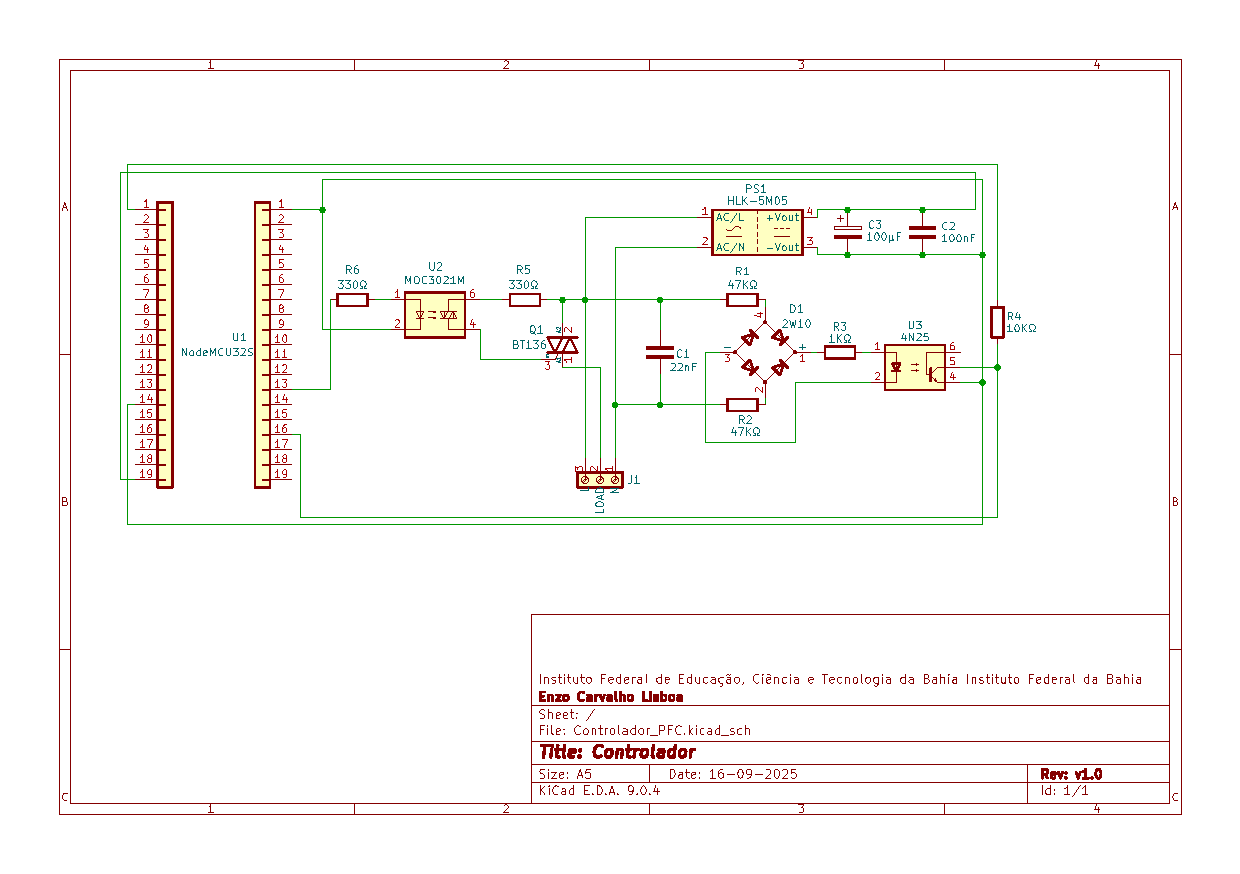
\includegraphics[angle=90, width=15.4cm]{./arquivos/Controlador.pdf} % PDF, PNG, JPG
   \caption{Projeto do circuito do controlador}
   \label{fig:proj_contr}
\end{figure}

\begin{figure}[htb]
   \centering
   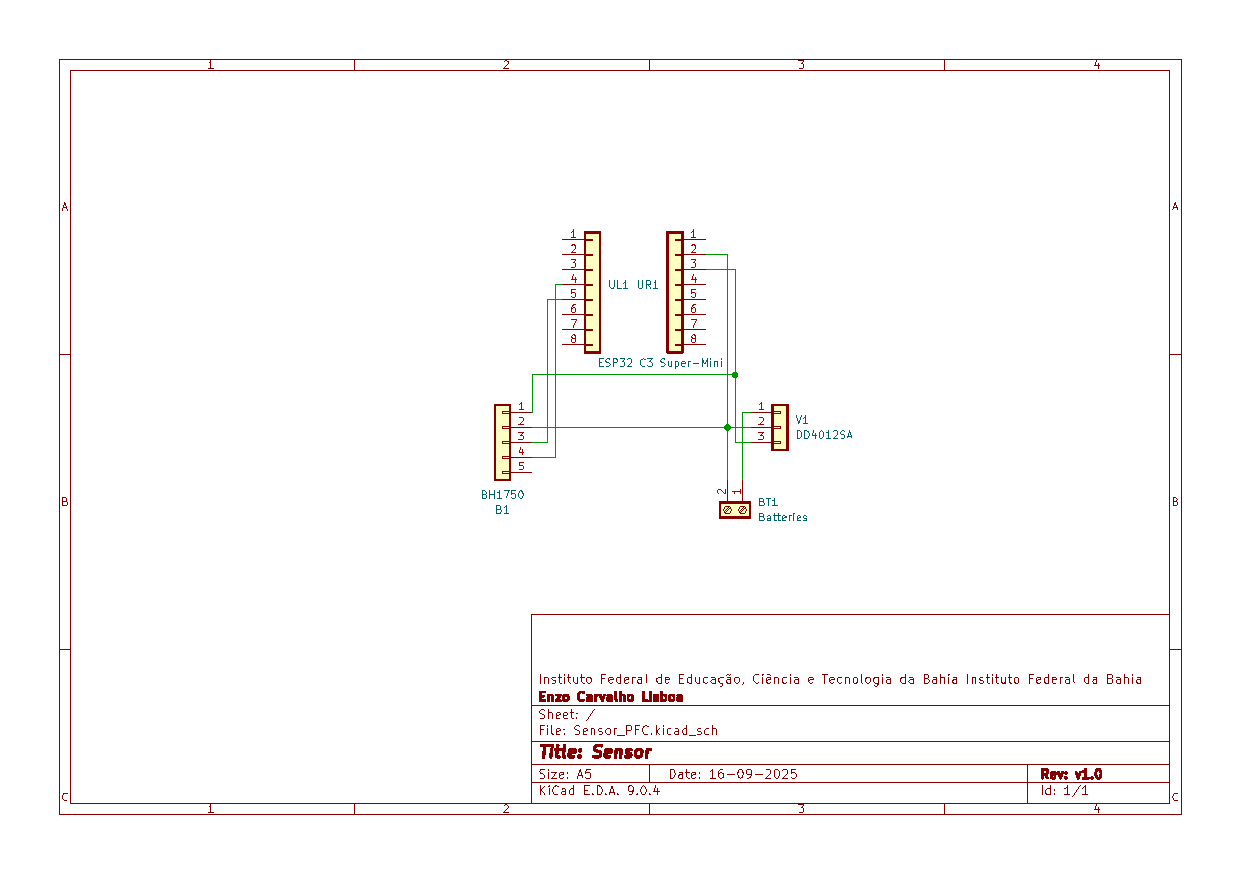
\includegraphics[angle=90, width=15.4cm]{./arquivos/Sensor.pdf} % PDF, PNG, JPG
   \caption{Projeto do circuito do sensor}
   \label{fig:proj_sens}
\end{figure}

\fi 
%
%%%%%%%%%%%%%%%%%%%%%%%%%%%%
%%%%%%%%%% AQUI VÃO SEUS ANEXOS  %%%%%%%%%%%%%%
%%%%%%%%%%%%%%%%%%%%%%%%%%%%
% ANEXOS são documentos criados por terceiros, e usados pelo autor (ABNT NBR14724)
%
% Apenas para PFC
%
\ifpfc % se é PFC
    %%%%%%%%%%%%
\chapter*{ANEXOS}
\addcontentsline{toc}{chapter}{ANEXOS}

\fi 
%
%
%%%%%%%%%%%%%%%%%%%%%%%%%%%%
%%%%%%%%%%%%%%%%%%%%%%%%%%%%
%%%% ÍNDICE REMISSIVO
%
% Apenas para PFC
%
\ifpfc % se é PFC
    \clearpage\pagebreak\newpage
    \ifpdf\phantomsection\fi
    \renewcommand{\indexname}{ÍNDICE REMISSIVO}
    \addcontentsline{toc}{chapter}{\indexname}
    \printindex  % índice remissivo
\fi 
%
%%%%%%%%%%%%%%%%%%%%%%%%%%%%%%

